\section{Results}
\label{sec:ode_results}

We present the posterior results of fitting the original BAHAMAS baseline, our baseline with improved priors, and our extensions with metallicity, formation rate, and age; all using Stan. All models are run using 4 chains with 1500 iterations each, of which half are discarded for warmup. 

% BASELINE 
\subsection{Baseline}
\label{sec:ode_results_baseline}

We first fit the original baseline model from \citet{Shariff+others:2016} in Stan. 

\begin{figure}
\centering
	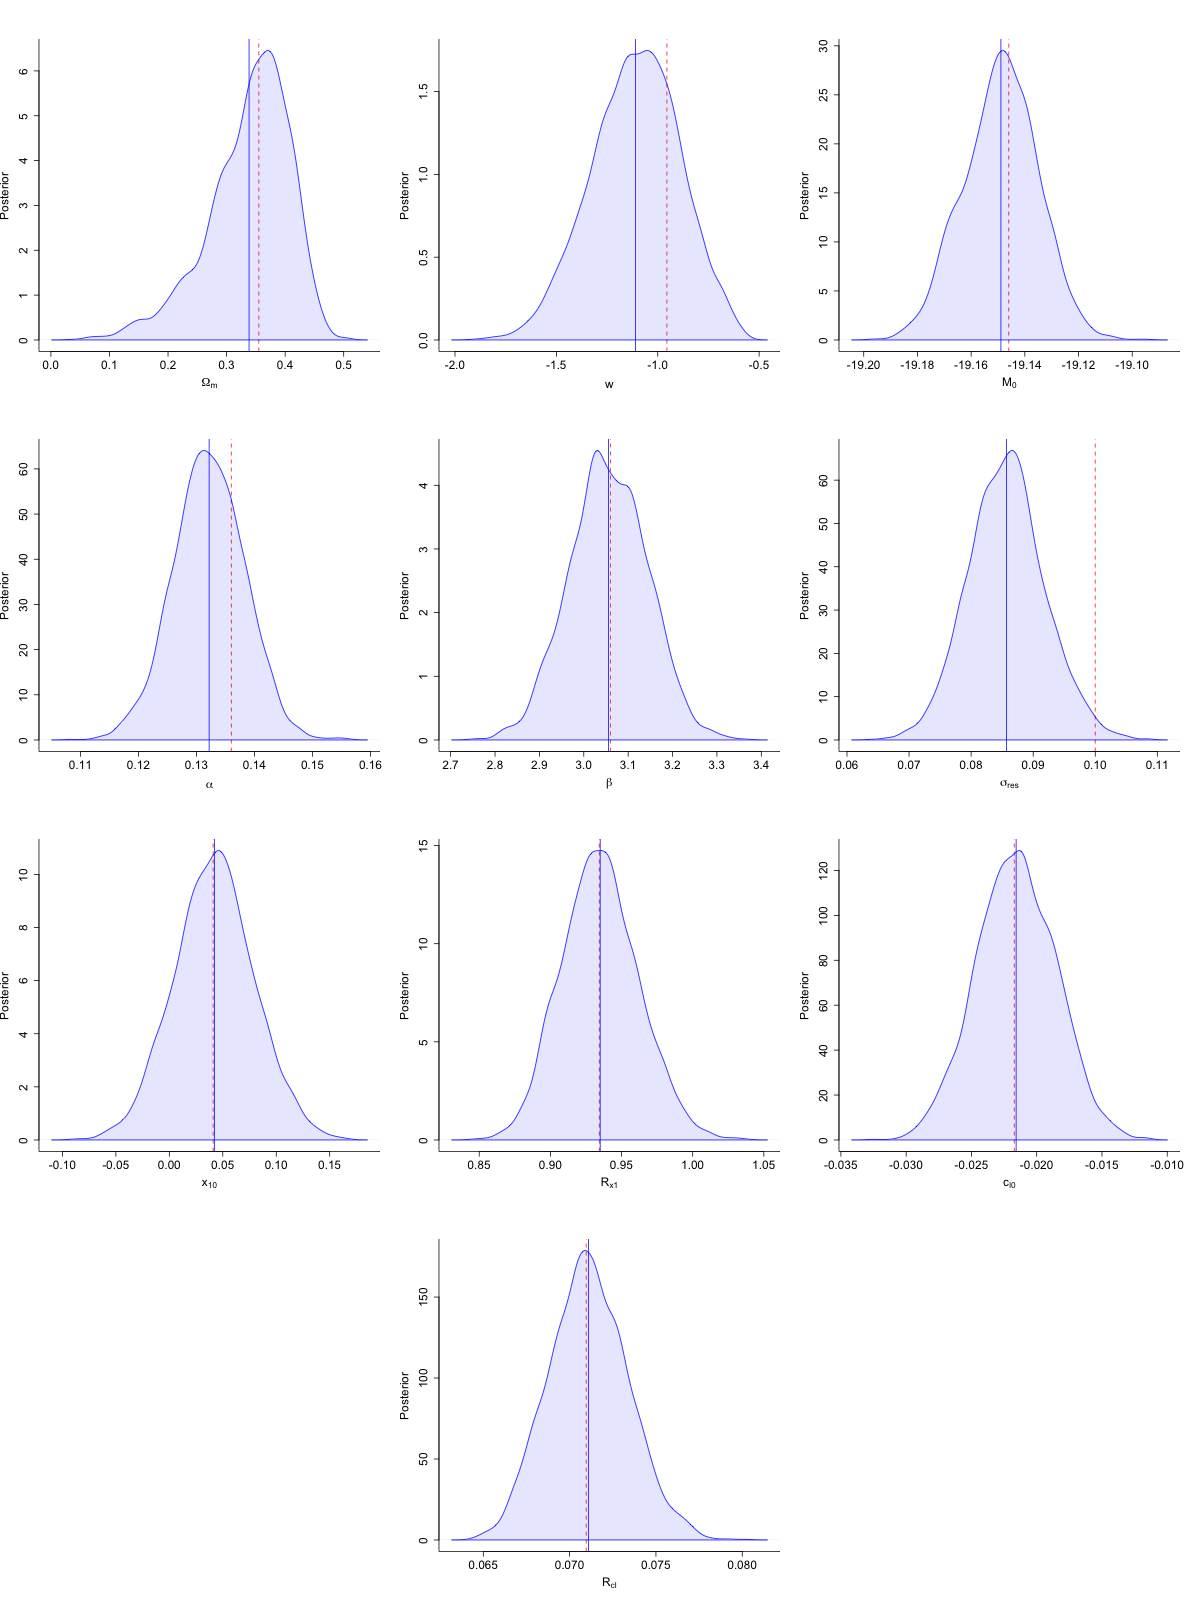
\includegraphics[width=0.9\textwidth]{figures/ode/base_flat_BAH_all.png}
\caption{Posterior distributions of the global parameters for the baseline (flat universe) model. Vertical blue lines correspond to posterior means while red lines correspond to BAHAMAS posterior means.}
\label{fig:ode_base_flat_BAH}
\end{figure}

Figure \ref{fig:ode_base_flat_BAH} displays the global parameter posteriors of the baseline model assuming a flat universe. Posterior means from the \citet{Shariff+others:2016} implementation are shown in red. While most of the parameters have similar posterior means, the $\sigma_{res}$ is quite off. This may be due to the original implementation using a more outdated set of values for the covariance matrix $\hat{C}$. Our results shown here use the latest values from the JLA study and are easily reproducible using our code. We believe the inconsistency in the $\hat{C}$, particularly with respect to the variance terms of $\hat{m}_B$, is also what prevents our cosmological parameters from lining up exactly with the BAHAMAS study. This is evidenced by the posterior means of $x_{10}, R_{x1}, c_{l0},$ and $R_{cl}$ matching perfectly with the \citet{Shariff+others:2016} posterior means.

\begin{figure}
\centering
	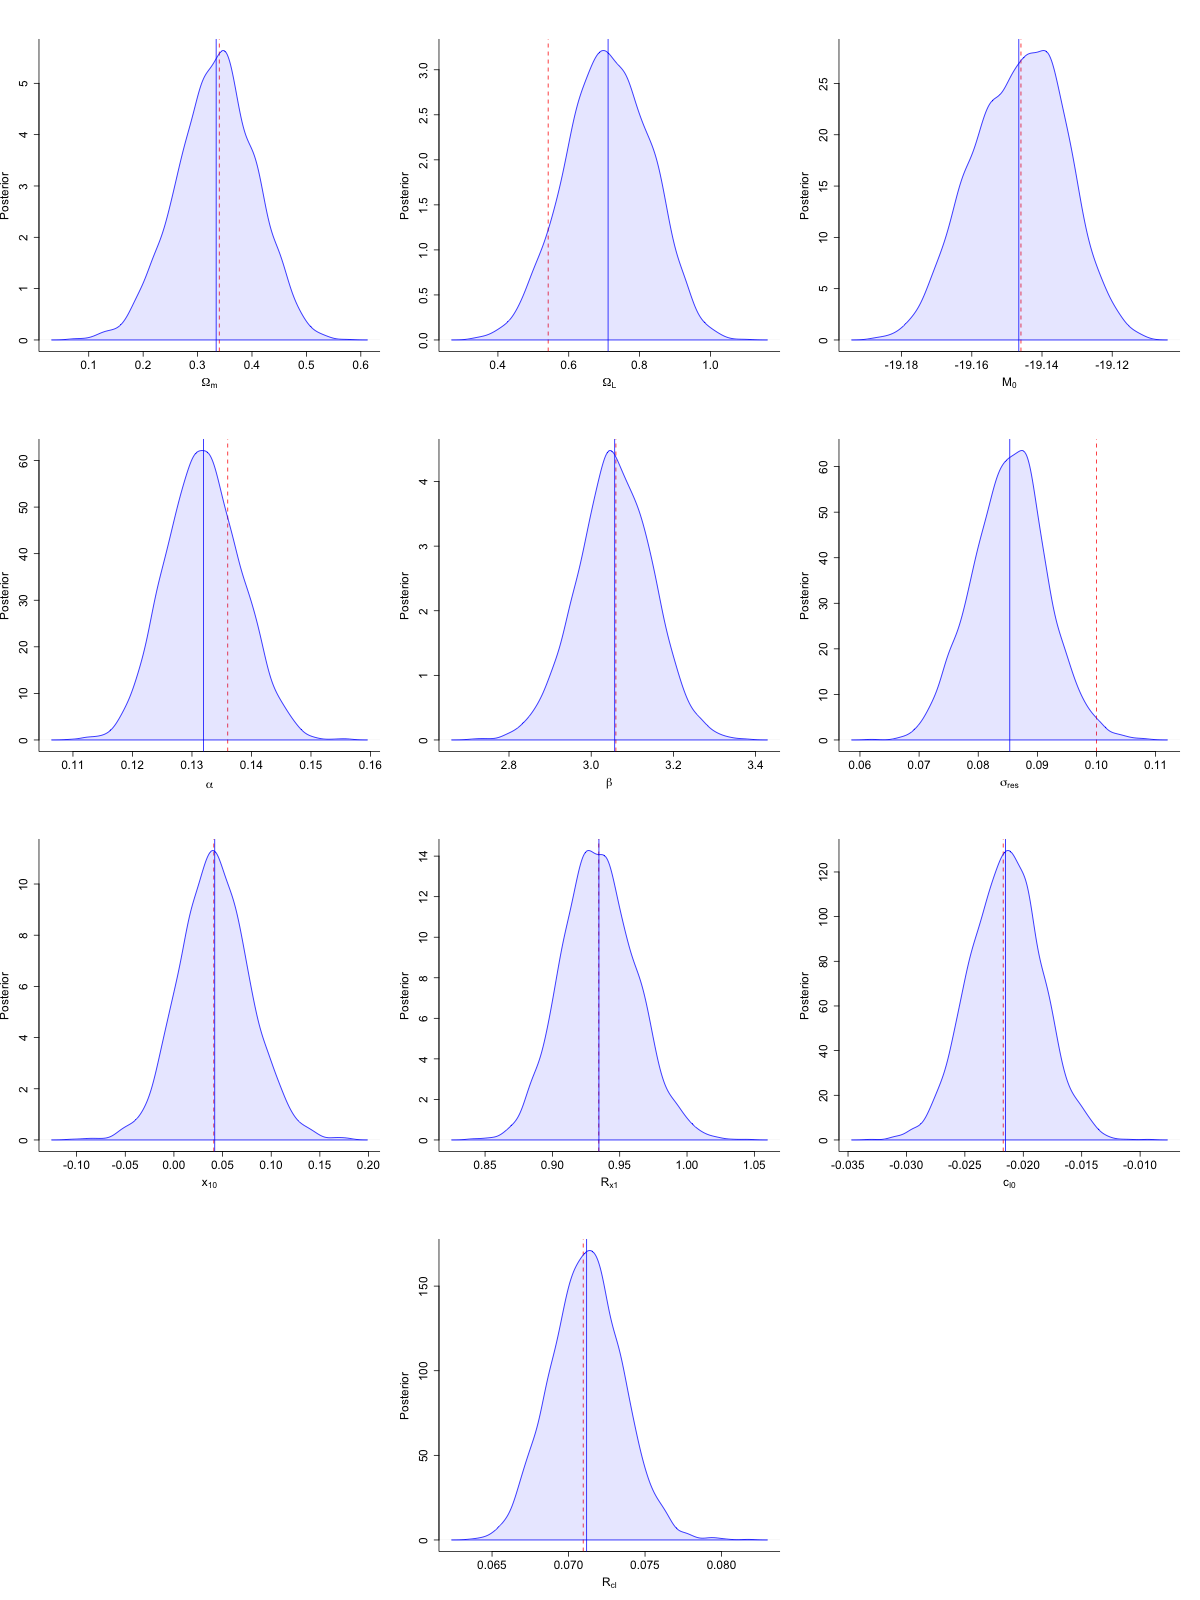
\includegraphics[width=0.9\textwidth]{figures/ode/base_curv_BAH_all.png}
\caption{Posterior distributions of the global parameters for the baseline (curved universe) model. Vertical blue lines correspond to posterior means while red lines correspond to BAHAMAS posterior means.}
\label{fig:ode_base_curv_BAH}
\end{figure}

Figure \ref{fig:ode_base_curv_BAH} displays the global parameter posteriors of the baseline model assuming a curved universe. The difference in posterior means between our implementation and the \citet{Shariff+others:2016} implementation are similar to those for the flat universe. Namely, the posterior distributions of $\beta, x_{10}, R_{x1}, c_{l0},$ and $R_{cl}$ are nearly identical to those arrived at by \citet{Shariff+others:2016}. However the posteriors of $\sigma_{res}, \alpha, \Omegam$, and $\OmegaL$ are quite different. Again, the difference in these latter four parameters is due the difference in the values of $\hat{C}$.

Aside from the technical issues behind the choice of the covariance matrix $\hat{C}$, there is no other reason to believe a Metropolis or Gibbs sampler would arrive to such starkly different posterior distributions as a NUTS or HMC sampler would. With that in mind, for the remaining model extensions we compare the newer models' posteriors to our own baseline posteriors for the curved and flat universe assumptions. This allows us to focus on the incremental impact of model choice rather than issues arising from data consistency. 

% BASELINE NEW PRIOR
\subsection{Baseline with new priors}
\label{sec:ode_results_baseline_new_prior}

We next present the results of adjusting the priors of the baseline model, as specified in Section \ref{sec:ode_new_priors}.

\begin{figure}
\centering
	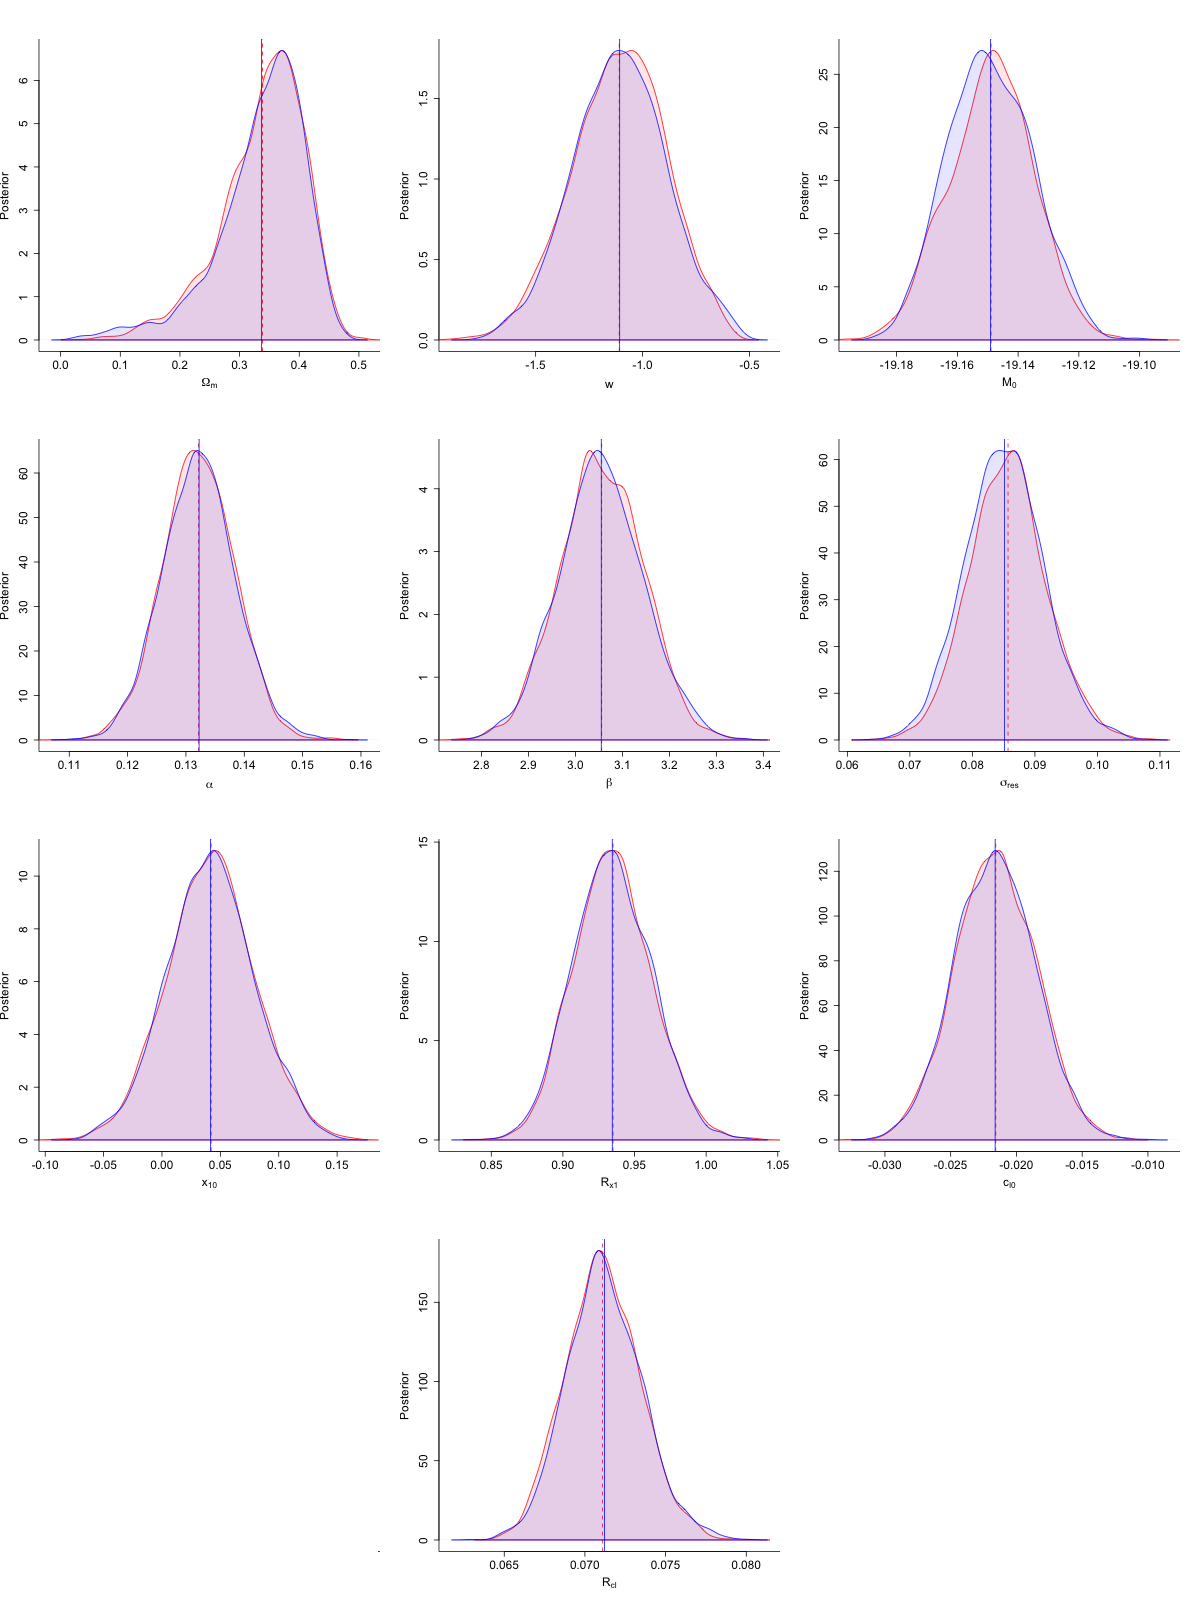
\includegraphics[width=0.9\textwidth]{figures/ode/base_flat_all.png}
\caption{Posterior distributions of the global parameters for the baseline (flat universe) model with new priors. Results from the older priors are shown in red. Vertical lines correspond to posterior means.}
\label{fig:ode_base_flat}
\end{figure}

Figure \ref{fig:ode_base_flat} displays the global parameter posteriors when using new priors for the baseline model assuming a flat universe. The posteriors resulting from the \citet{Shariff+others:2016} priors are shown in red. The posteriors are nearly identical, showing that the results aren't sensitive to the prior choice.

\begin{figure}
\centering
	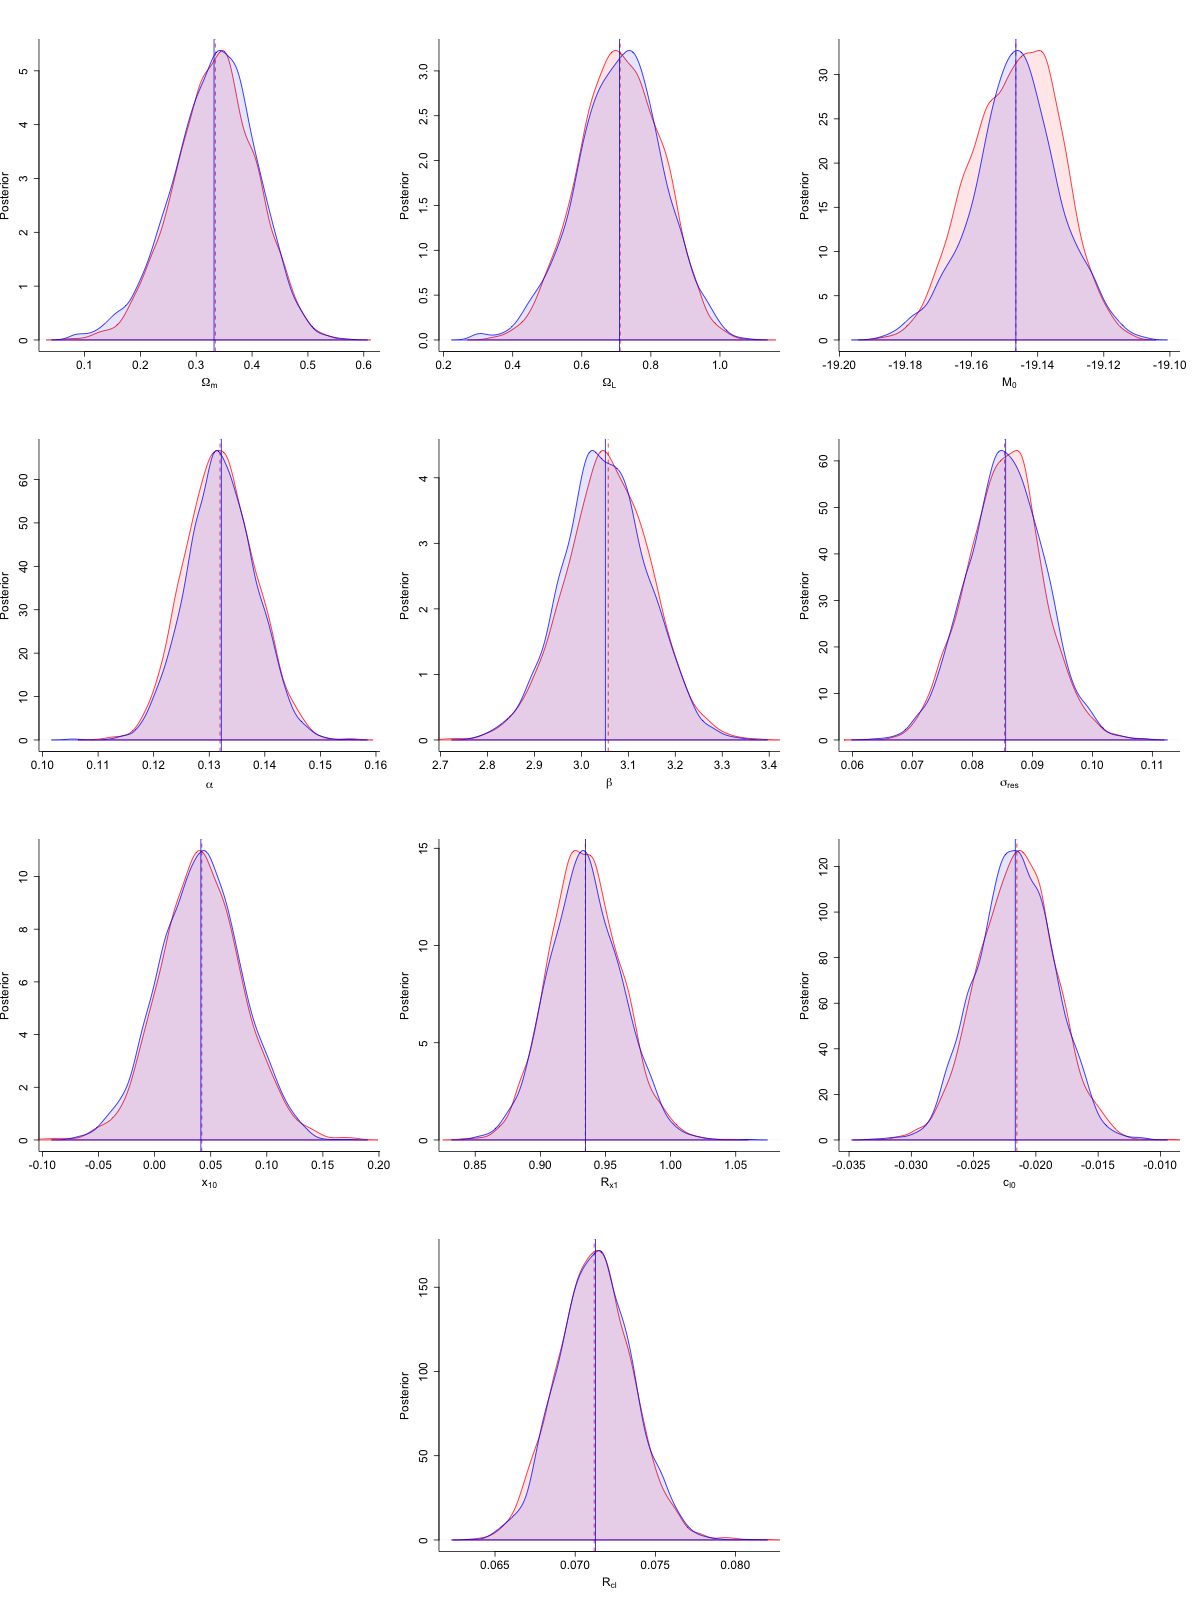
\includegraphics[width=0.9\textwidth]{figures/ode/base_curv_all.png}
\caption{Posterior distributions of the global parameters for the baseline (curved universe) model with new priors. Results from the older priors are shown in red. Vertical lines correspond to posterior means.}
\label{fig:ode_base_curv}
\end{figure}

Figure \ref{fig:ode_base_curv} displays the global parameter posteriors when using new priors for the baseline model assuming a curved universe. The posteriors resulting from the \citet{Shariff+others:2016} priors are shown in red. The posteriors are nearly identical for the curved universe as well, showing that the results aren't sensitive to the prior choice.

For the remaining three model extensions, we omit the posterior results for $x_{10}, R_{x1}, c_{l0}$, and $R_{cl}$ since these global parameters are unaffected by inclusion of a third covariate. 

% STAR METALLICITY
\subsection{Star metallicity}
\label{sec:ode_results_metallicity}

We next present the results of adding star stametallicity to the baseline model with new priors. Comparisons are made to the posteriors resulting from fitting the baseline model with new priors, as in Section \ref{sec:ode_results_baseline_new_prior}. Here $\alpha_1$ and $\beta_1$ correspond to the stretch and color correction regression coefficients learned from the subset of 113 supernovae from the Campbell study, which are entered into the likelihood via (\ref{eq:metallicity_likelihood}). Additionally, $\gamma_{m}$ is the star metallicity regression coefficient learned from the Campbell supernovae subset. Meanwhile, $\alpha$ and $\beta$ correspond to regression coefficients learned from the remaining 627 supernovae, which are entered into the likelihood via (\ref{eq:baseline_likelihood}). The remaining parameters are shared in the likelihood by both subsets of supernovae. 

\begin{figure}
\centering
	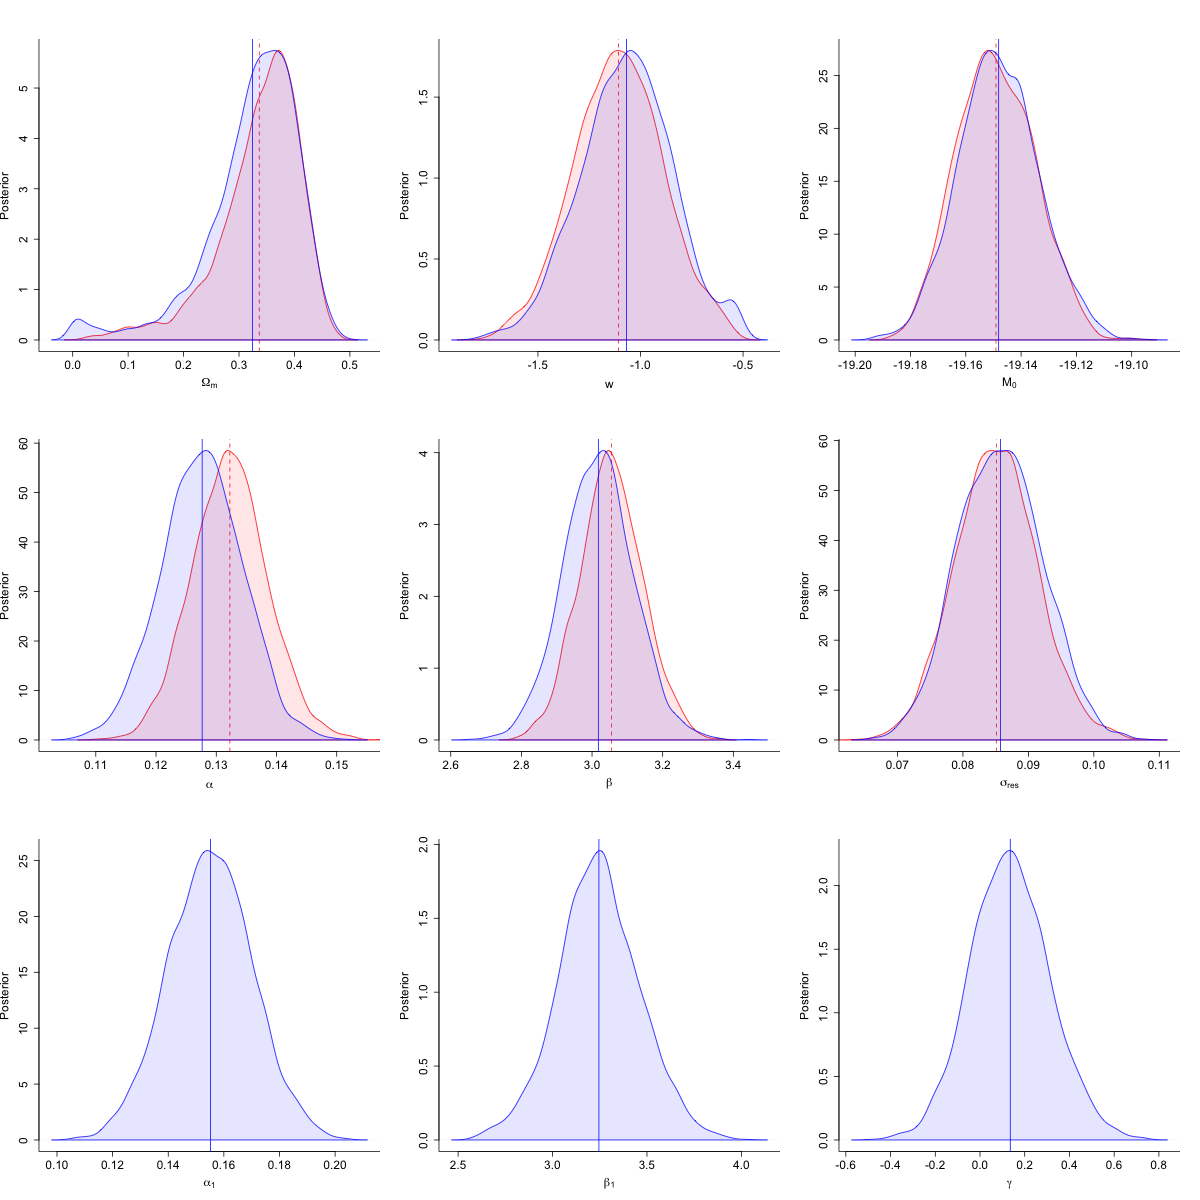
\includegraphics[width=0.9\textwidth]{figures/ode/split_meth_flat_camp.png}
\caption{Posterior distributions of the global parameters for the baseline (flat universe) model with new priors and metallicity. Results without metallicity are shown in red. Vertical lines correspond to posterior means.}
\label{fig:ode_meth_flat}
\end{figure}

Figure \ref{fig:ode_meth_flat} displays the global parameter posteriors when using new priors for the baseline model assuming a flat universe, and adding star metallicity as a covariate. The posteriors resulting from the new priors without metallicity are shown in red. The global shared parameters $\Omegam, \OmegaL, M_0,$ and $\sigma_{res}$ are relatively unchanged by the addition of metallicity as a covariate, while the regression parameters $\alpha$ and $\beta$ are changed primarily because they are learned from a subset of 627 supernovae, as opposed to all 740. Most crucially, however, the posterior of $\gamma_{m}$ contains 0 even in its central 50\% interval, suggesting that star metallicity does not help reduce the variation with which we can estimate the cosmological parameters.

\begin{figure}
\centering
	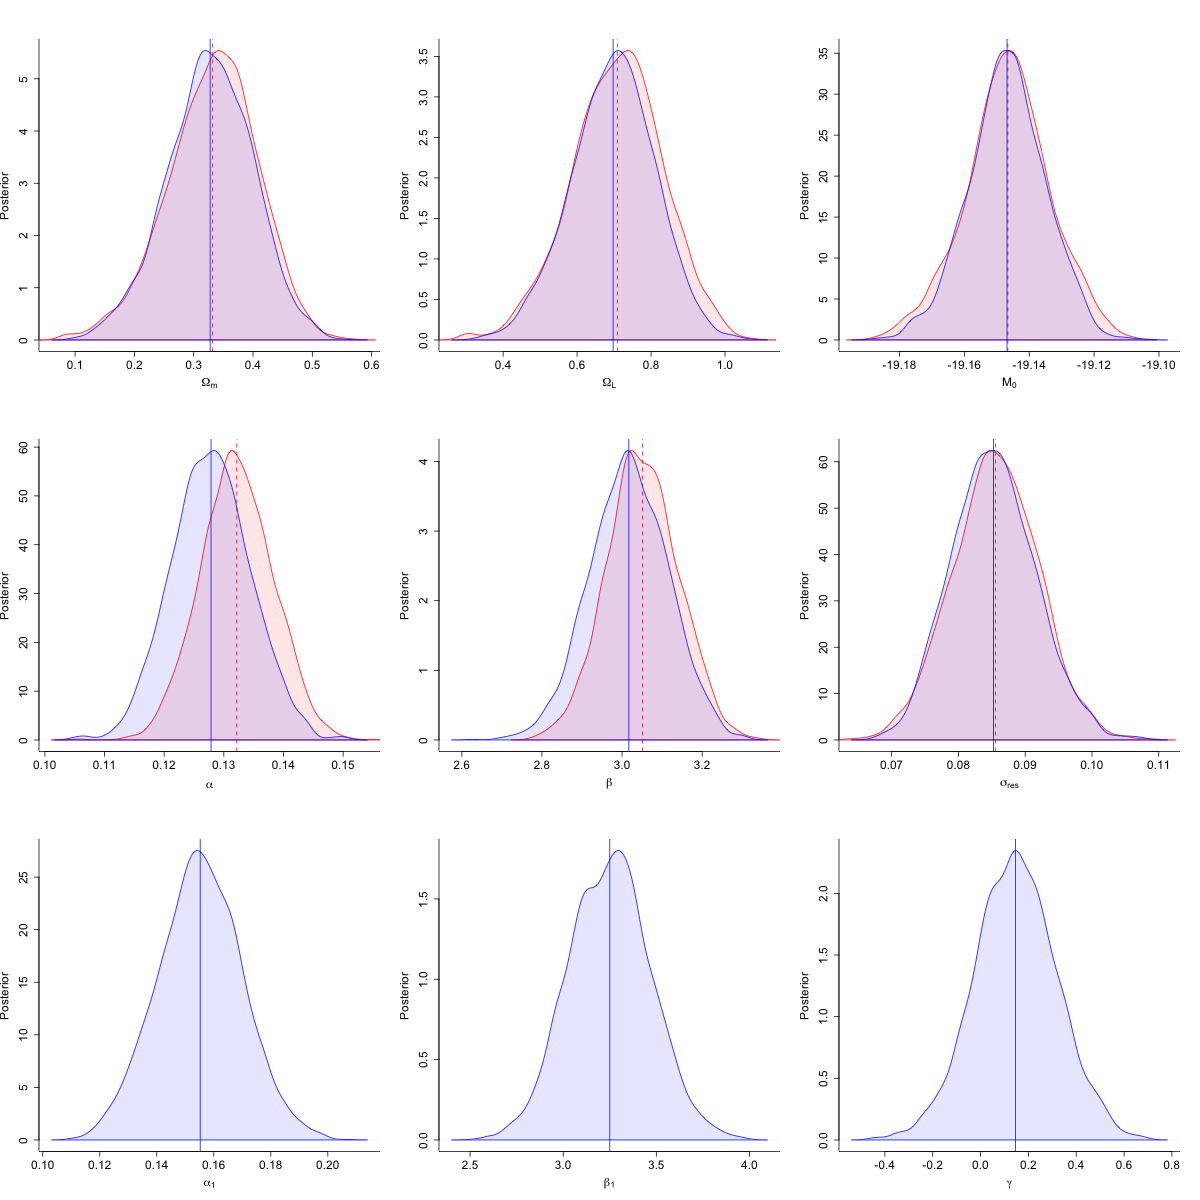
\includegraphics[width=\textwidth]{figures/ode/split_meth_curv_camp.png}
\caption{Posterior distributions of the global parameters for the baseline (curved universe) model with new priors and metallicity. Results without metallicity are shown in red. Vertical lines correspond to posterior means.}
\label{fig:ode_meth_curv}
\end{figure}

Figure \ref{fig:ode_meth_curv} displays the global parameter posteriors when using new priors for the baseline model assuming a curved universe, and adding star metallicity as a covariate. The posteriors resulting from the new priors without metallicity are shown in red. As under the flat universe assumption, the posterior of $\gamma_{m}$ contains 0 even in its central 50\% interval, suggesting that star metallicity does not help reduce the variation with which we can estimate the cosmological parameters.

% STAR FORMATION RATE
\subsection{Star formation rate}
\label{sec:ode_results_rate}

We next present the results of adding star formation rate to the baseline model with new priors. Comparisons are made to the posteriors resulting from fitting the baseline model with new priors, as in Section \ref{sec:ode_results_baseline_new_prior}. Here $\alpha_1$ and $\beta_1$ correspond to the stretch and color correction regression coefficients learned from the subset of 113 supernovae from the Campbell study, which are entered into the likelihood via (\ref{eq:formation_likelihood}). Additionally, $\gamma_{f}$ is the star formation rate regression coefficient learned from the Campbell supernovae subset. Meanwhile, $\alpha$ and $\beta$ correspond to regression coefficients learned from the remaining 627 supernovae, which are entered into the likelihood via (\ref{eq:baseline_likelihood}). The remaining parameters are shared in the likelihood by both subsets of supernovae. 

\begin{figure}
\centering
	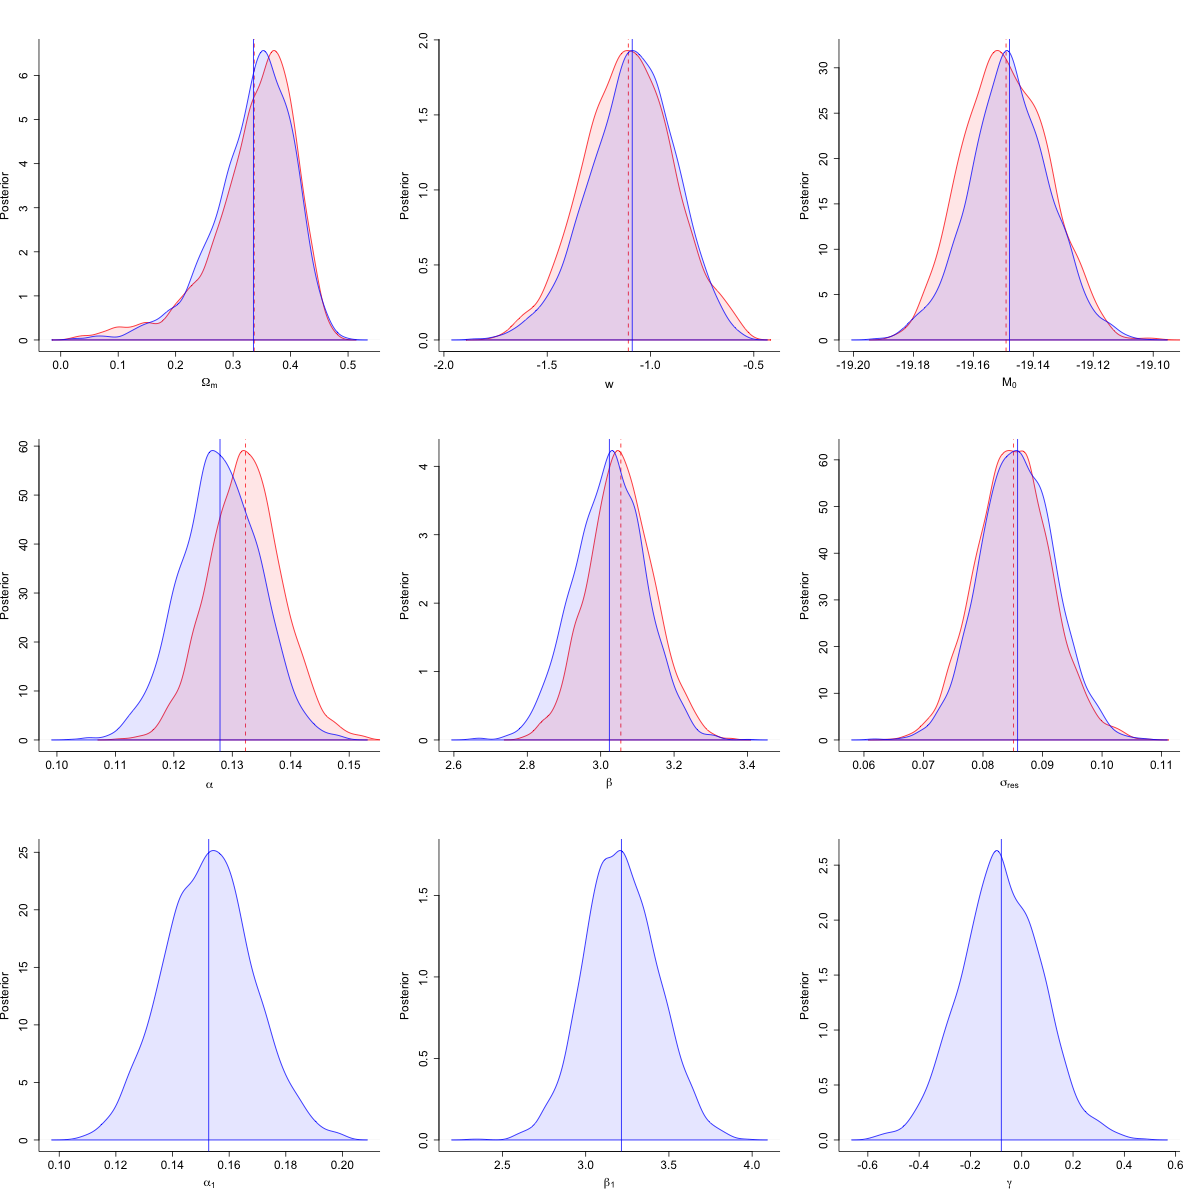
\includegraphics[width=\textwidth]{figures/ode/split_rate_flat_camp.png}
\caption{Posterior distributions of the global parameters for the baseline (flat universe) model with new priors and formation rate. Results without formation rate are shown in red. Vertical lines correspond to posterior means.}
\label{fig:ode_rate_flat}
\end{figure}

Figure \ref{fig:ode_rate_flat} displays the global parameter posteriors when using new priors for the baseline model assuming a flat universe, and adding star formation rate as a covariate. The posteriors resulting from the new priors without metallicity are shown in red. The posterior of $\gamma_{f}$ contains 0 even in its central 50\% interval, suggesting that star formation rate does not help reduce the variation with which we can estimate the cosmological parameters.

\begin{figure}
\centering
	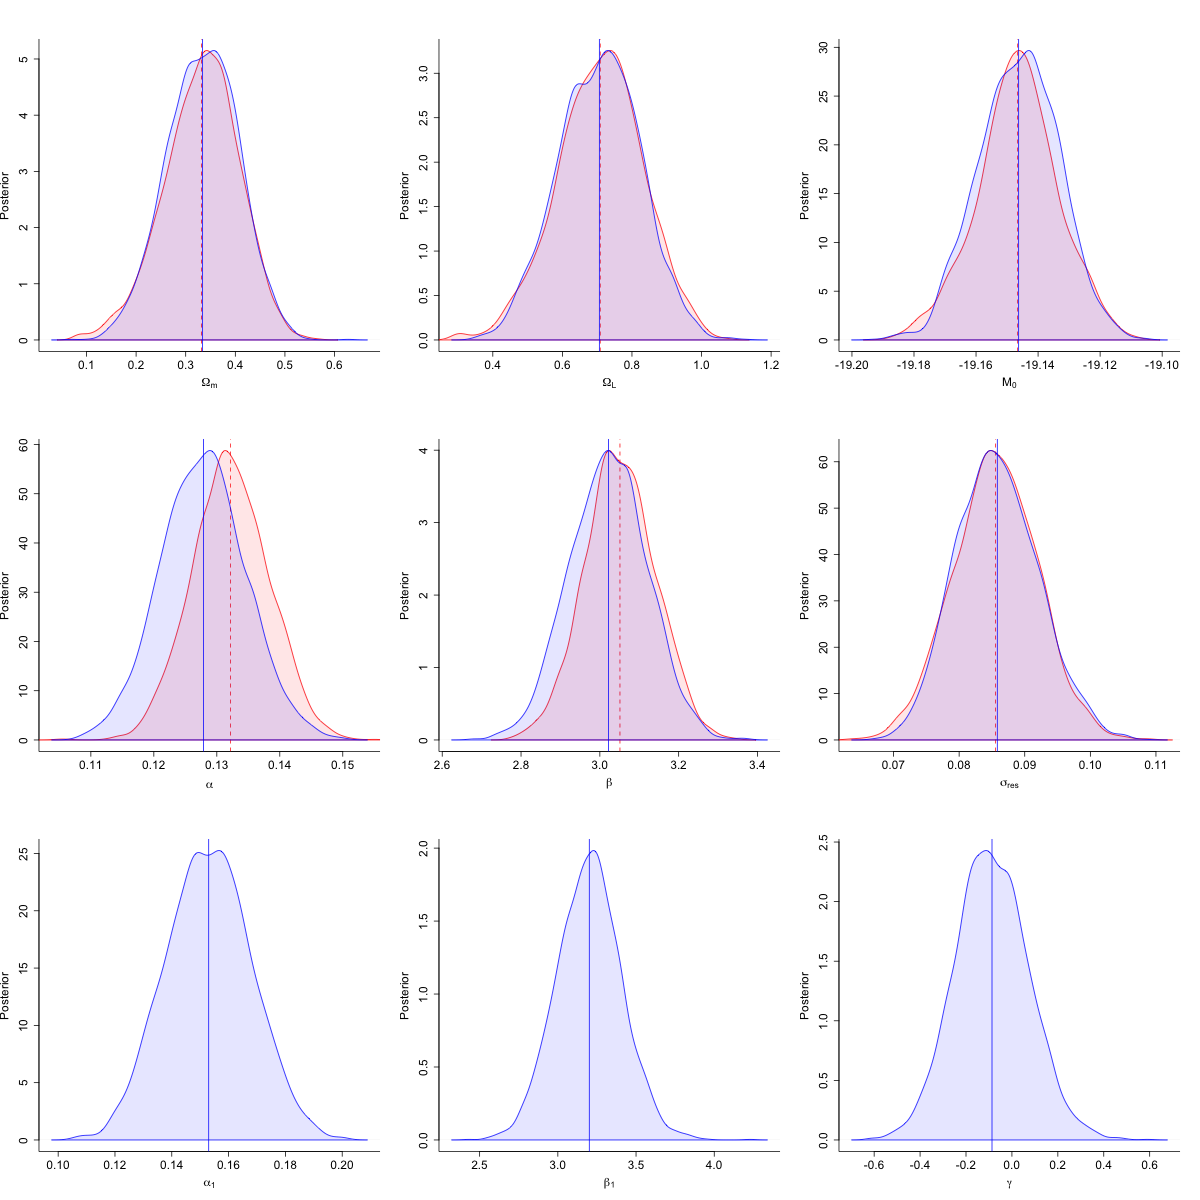
\includegraphics[width=\textwidth]{figures/ode/split_rate_curv_camp.png}
\caption{Posterior distributions of the global parameters for the baseline (curved universe) model with new priors and formation rate. Results without formation rate are shown in red. Vertical lines correspond to posterior means.}
\label{fig:ode_rate_curv}
\end{figure}

Figure \ref{fig:ode_rate_curv} displays the global parameter posteriors when using new priors for the baseline model assuming a curved universe, and adding star formation rate as a covariate. The posteriors resulting from the new priors without metallicity are shown in red. As under the flat universe assumption, the posterior of $\gamma_{f}$ contains 0 even in its central 50\% interval, suggesting that star formation rate does not help reduce the variation with which we can estimate the cosmological parameters.

% GALAXY AGE
\subsection{Galaxy age}
\label{sec:ode_results_age}

We next present the results of adding galaxy age to the baseline model with new priors. Comparisons are made to the posteriors resulting from fitting the baseline model with new priors, as in Section \ref{sec:ode_results_baseline_new_prior}. Here $\alpha_1$ and $\beta_1$ correspond to the stretch and color correction regression coefficients learned from the subset of 113 supernovae from the Campbell study, which are entered into the likelihood via (\ref{eq:age_likelihood}). Additionally, $\gamma_{a}$ is the galaxy age coefficient learned from the Campbell supernovae subset. Meanwhile, $\alpha$ and $\beta$ correspond to regression coefficients learned from the remaining 627 supernovae, which are entered into the likelihood via (\ref{eq:baseline_likelihood}). The remaining parameters are shared in the likelihood by both subsets of supernovae. 

\begin{figure}
\centering
	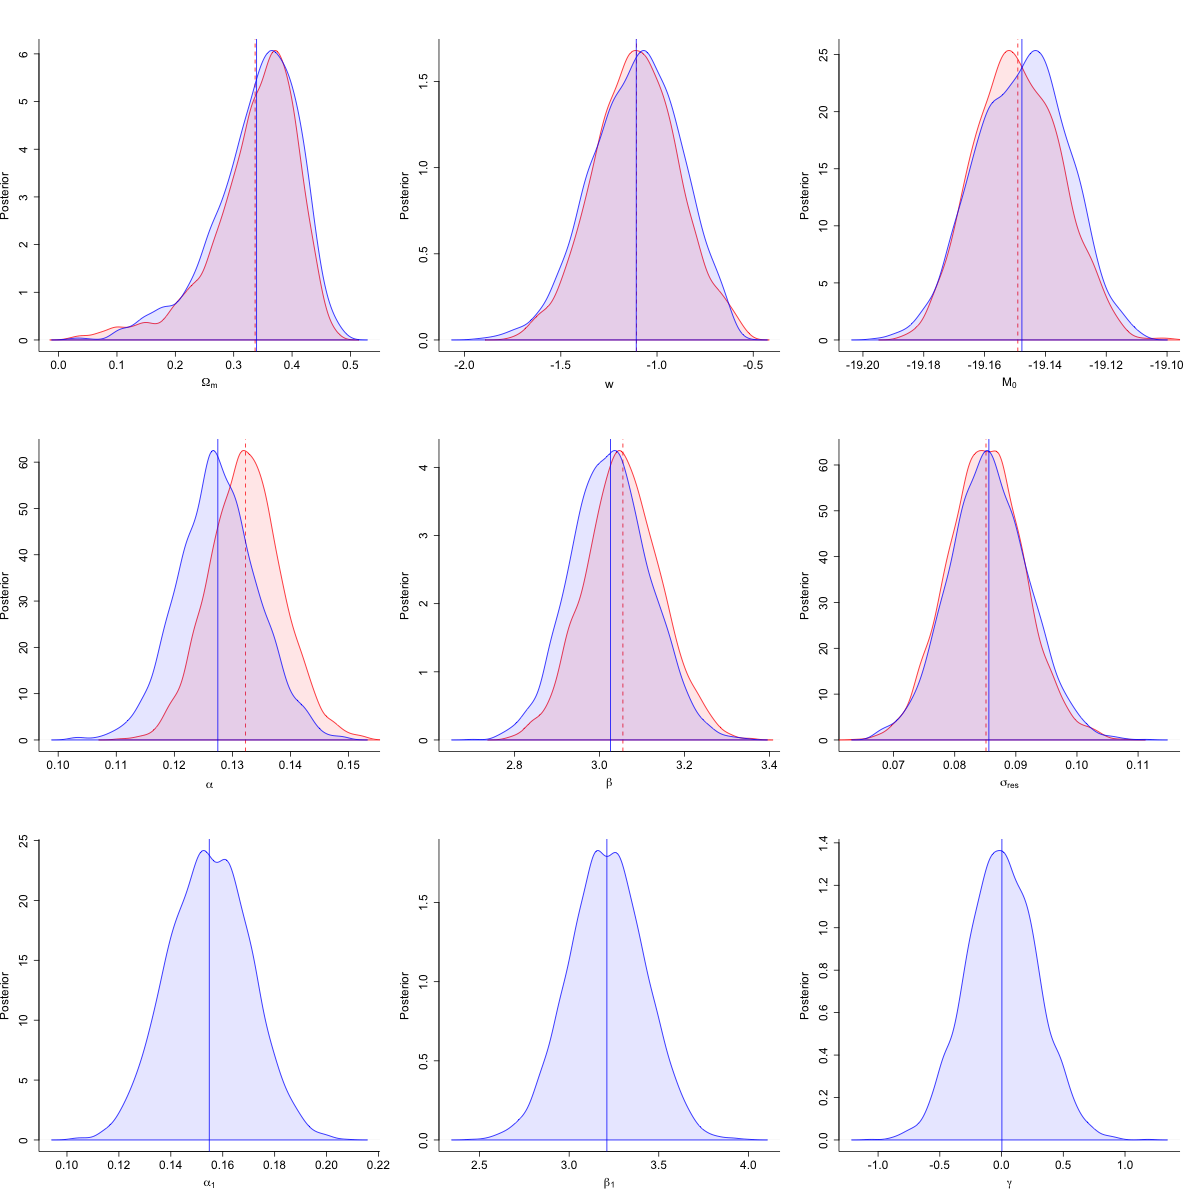
\includegraphics[width=\textwidth]{figures/ode/split_age_flat_camp.png}
\caption{Posterior distributions of the global parameters for the baseline (flat universe) model with new priors and age. Results without age are shown in red. Vertical lines correspond to posterior means.}
\label{fig:ode_age_flat}
\end{figure}

Figure \ref{fig:ode_age_flat} displays the global parameter posteriors when using new priors for the baseline model assuming a flat universe, and adding galaxy age as a covariate. The posteriors resulting from the new priors without metallicity are shown in red. The posterior of $\gamma_{a}$ is essentially 0, suggesting that galaxy age does not help reduce the variation with which we can estimate the cosmological parameters.

\begin{figure}
\centering
	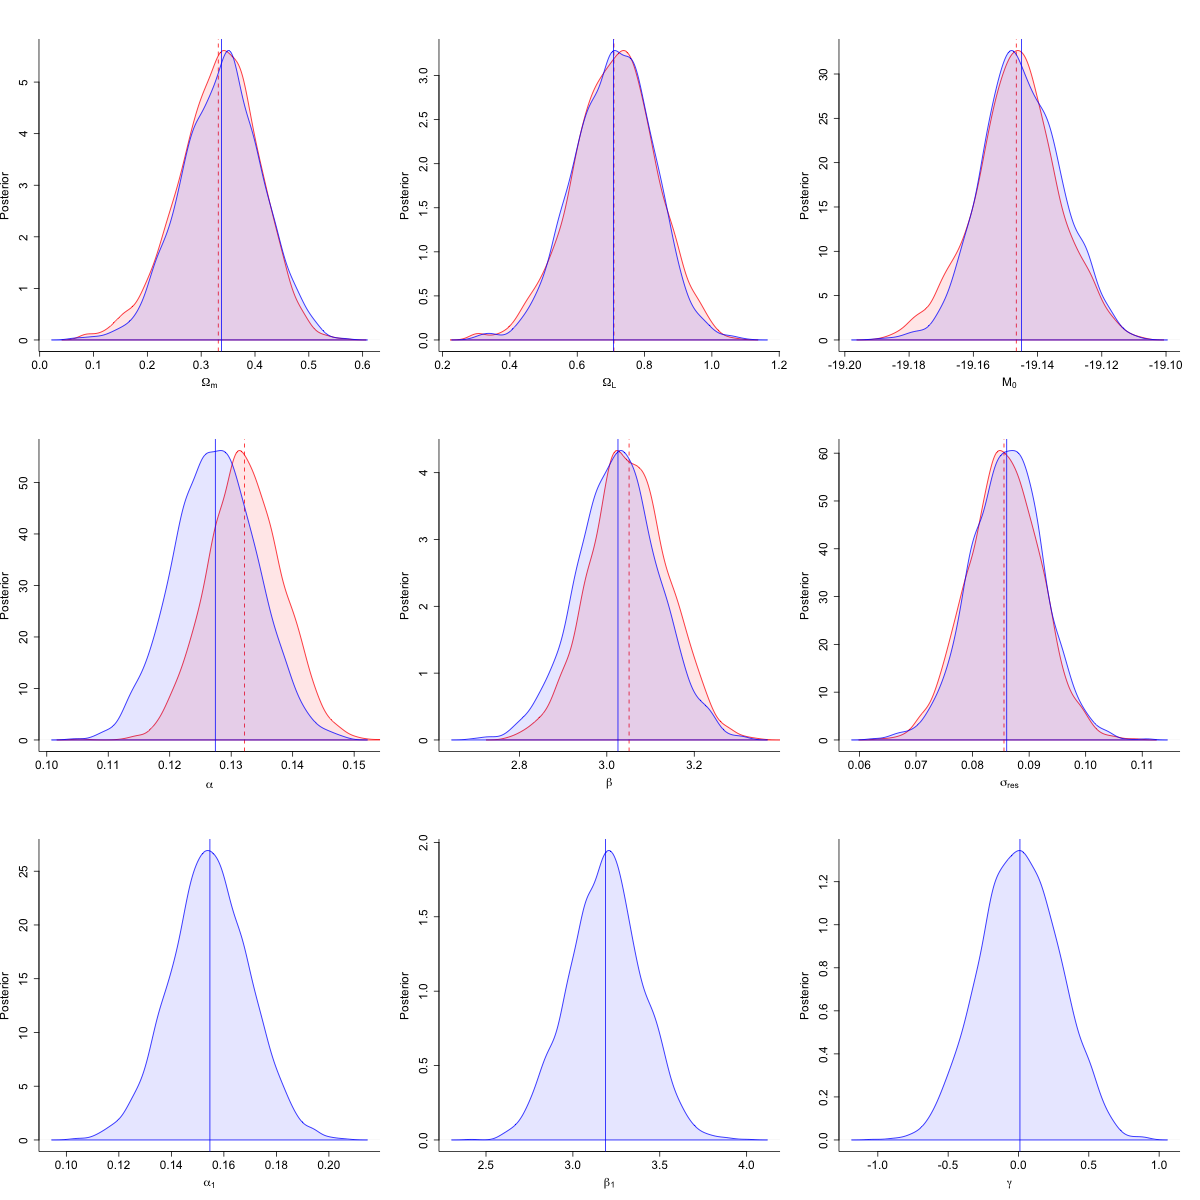
\includegraphics[width=\textwidth]{figures/ode/split_age_curv_camp.png}
\caption{Posterior distributions of the global parameters for the baseline (curved universe) model with new priors and age. Results without age are shown in red. Vertical lines correspond to posterior means.}
\label{fig:ode_age_curv}
\end{figure}

Figure \ref{fig:ode_age_curv} displays the global parameter posteriors when using new priors for the baseline model assuming a curved universe, and adding galaxy age as a covariate. The posteriors resulting from the new priors without metallicity are shown in red. As under the flat universe assumption, the posterior mean of $\gamma_{a}$ is essentially 0, suggesting that galaxy age does not help further reduce the variation with which we can estimate the cosmological parameters.

